

\subsection{Specifying the Plotted Range}

\begin{pgfplotsxykeylist}{\x min=\marg{coord},\x max=\marg{coord}}
The options |xmin|, |xmax| and |ymin|, |ymax| allow to define the axis limits, i.e.\ the lower left and the upper right corner. Everything outside of the axis limits will be clipped away.

Each missing limit will be determined automatically.

If $x$-limits have been specified explicitly and $y$-limits are computed automatically, the automatic computation of $y$-limits will only considers points which fall into the specified $x$-range (and vice--versa). The same holds true if, for example, only |xmin| has been provided explicitly: in that case, |xmax| will be updated only for points for which $x \ge $|xmin| holds. This feature can be disabled using |clip limits=false|. 

Axis limits can be increased automatically using the |enlargelimits| option.
\begin{codeexample}[]
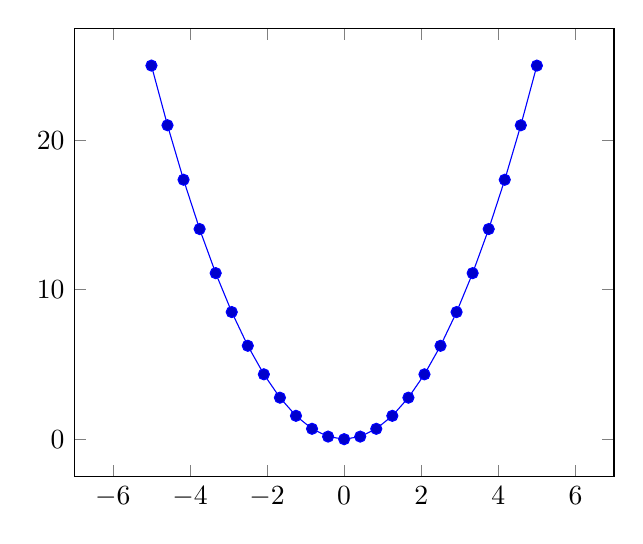
\begin{tikzpicture}
	\begin{axis}
	\addplot {x^2};
	\end{axis}
\end{tikzpicture}
\end{codeexample}

\begin{codeexample}[]
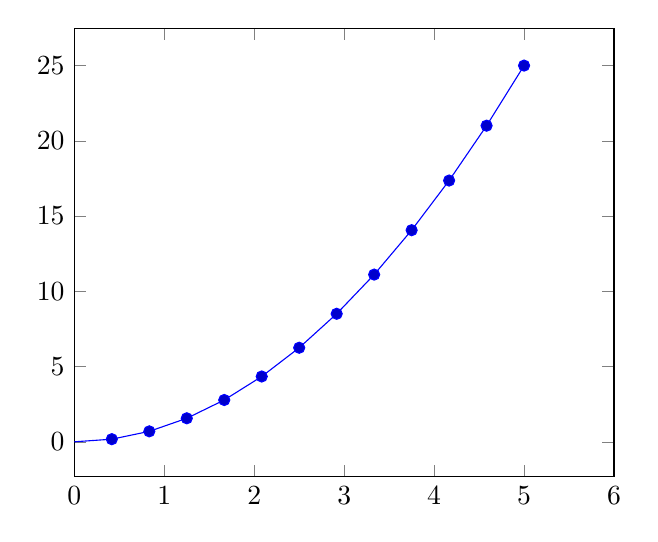
\begin{tikzpicture}
	\begin{axis}[xmin=0]
	\addplot {x^2};
	\end{axis}
\end{tikzpicture}
\end{codeexample}

\begin{codeexample}[]
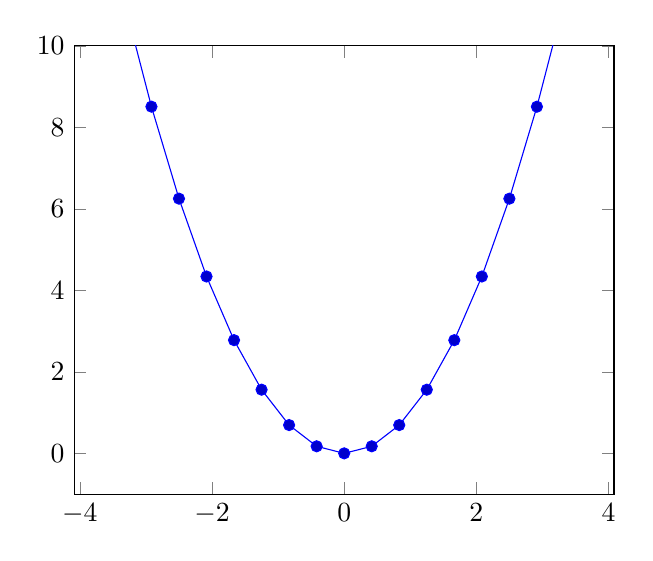
\begin{tikzpicture}
	\begin{axis}[ymax=10]
	\addplot {x^2};
	\end{axis}
\end{tikzpicture}
\end{codeexample}
\end{pgfplotsxykeylist}

\begin{pgfplotsxykey}{\x mode=\mchoice{normal,linear,log} (initially normal)}
	Allows to choose between linear (=normal) or logarithmic axis scaling or logplots for each $x,y,z$-combination.

	Logarithmic plots use the current setting of |log basis x| and its variants to determine the basis (default is $e$).
	% FIXME : replicated in pgfplots.reference.scaling.tex
\end{pgfplotsxykey}

\begin{pgfplotsxykey}{\x\ dir=\mchoice{normal,reverse} (initially normal)}
\pgfkeys{/pdflinks/search key prefixes in/.add={/pgfplots/,}{}}
	Allows to revert axis directions such that values are given in decreasing order.
\label{key:pgfplots:xydir}
\begin{codeexample}[]
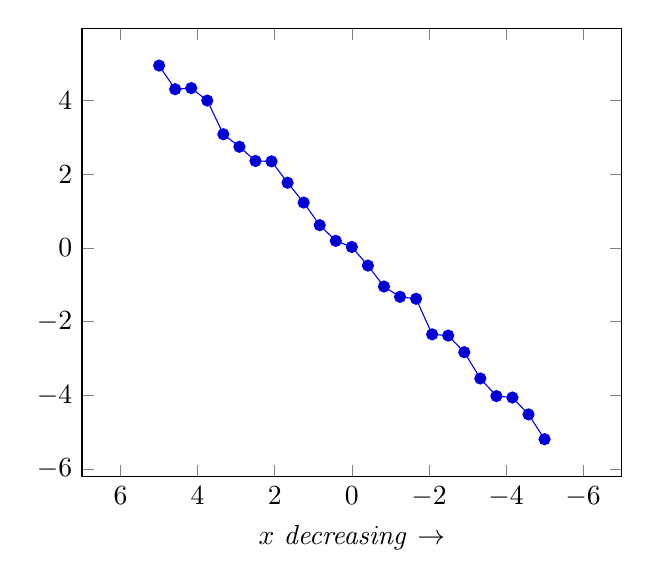
\begin{tikzpicture}
\begin{axis}[
	xlabel=$x$ \emph{decreasing} $\to$,
	x dir=reverse]
	\addplot {x+rand*0.3};
\end{axis}
\end{tikzpicture}
\end{codeexample}

\begin{codeexample}[]
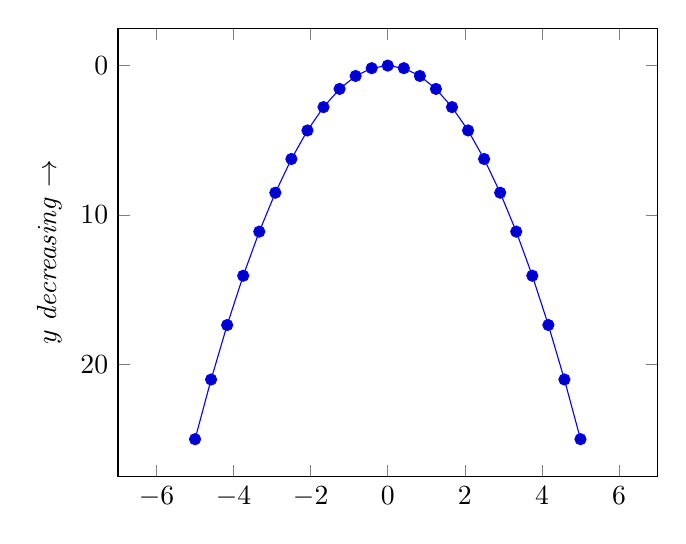
\begin{tikzpicture}
\begin{axis}[
	ylabel=$y$ \emph{decreasing} $\to$,
	y dir=reverse]
	\addplot {x^2};
\end{axis}
\end{tikzpicture}
\end{codeexample}

	Note, that axis descriptions and relative positioning macros will stay at the same place as they would for non--reversed axes.
\begin{codeexample}[]
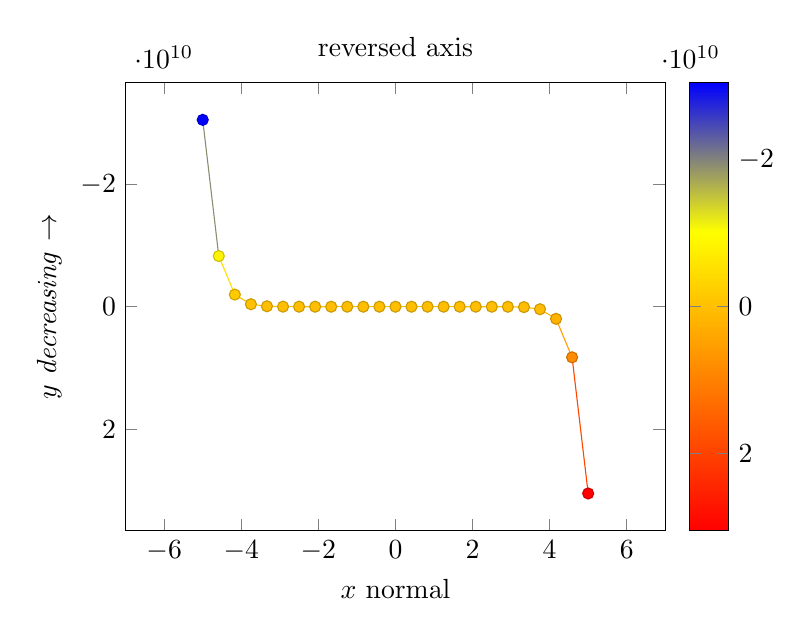
\begin{tikzpicture}
\begin{axis}[
	ylabel=$y$ \emph{decreasing} $\to$,
	xlabel=$x$ normal,
	title=reversed axis,
	y dir=reverse,
	colorbar,
	colorbar style={y dir=reverse}]
	\addplot+[mesh,scatter] {x^15};
\end{axis}
\end{tikzpicture}
\end{codeexample}

	Note that |colorbar|s won't be reversed automatically, you will have to reverse the sequence of color bars manually in case this is required as in the preceding example.
\end{pgfplotsxykey}

\begin{pgfplotskey}{clip limits=\mchoice{true,false} (initially true)}
	Configures what to do if some, but not all axis limits have been specified explicitly. In case |clip limits=true|, the automatic limit computation will \emph{only} consider points which do not contradict the explicitly set limits. 

	This option has nothing to do with path clipping, it only affects how the axis limits are computed.
\end{pgfplotskey}

\begin{pgfplotsxykeylist}{enlarge \x\ limits=\mchoice{auto,true,false,upper,lower,\meta{val},value=\meta{val},abs value=\meta{val},\\ abs=\meta{val},rel=\meta{val}} (initially auto),
	enlargelimits=\meta{common value}}
Enlarges the axis size for one axis (or all of them for |enlargelimits|) somewhat if enabled.

You can set |xmin|, |xmax| and |ymin|, |ymax| to the minimum/maximum values of your data and |enlarge x limits| will enlarge the canvas such that the axis doesn't touch the plots.

\begin{itemize}
	\item The value \declaretext{true} enlarges the lower and upper limit.
	\item The value \declaretext{false} uses tight axis limits as specified by the user (or read from input coordinates).
	\item The value \declaretext{auto} will enlarge limits only for axis for which axis limits have been determined automatically.

	For threedimensional figures, the \declaretext{auto} mechanism applies only for the $z$ axis. The $x$ and $y$ axis won't be enlarged. 
	\item The value \declaretext{upper} enlarges only the upper axis limit while \declaretext{lower} enlarges only the lower axis limit.
	\item Values like `|enlarge x limits=0.1|' will enlarge lower and upper axis limit relatively (in this example, $10\%$ of the axis limits will be added on both sides).
	\item It is also possible to change just the relative threshold using the \declaretext{value=}\marg{val} key. It can be combined with any of the other possible values. For example, 

		|\pgfplotsset{enlarge x limits={value=0.2,upper}}|
	
	will enlarge (only) the upper axis limit by $20\%$ of the axis range. Another example is

		|\pgfplotsset{enlarge x limits={value=0.2,auto}}|

	which changes the default threshold of the \declaretext{auto} value to $20\%$.
	\item While |value| uses relative thresholds, \declaretext{abs value} is used in the same way with absolute values.

	\paragraph{Attention:} |abs value| is applied \emph{multiplicative} for logarithmic axes! That means |abs value=10| for a logarithmic axis adds $\log 10$ to upper and/or lower axis limits.

	\item Finally, \declaretext{abs=}\marg{value} is the same as |true,abs value=|\marg{value} and \declaretext{rel=}\marg{value} is the same as |true,value=|\marg{value}.
\end{itemize}
\begin{codeexample}[]
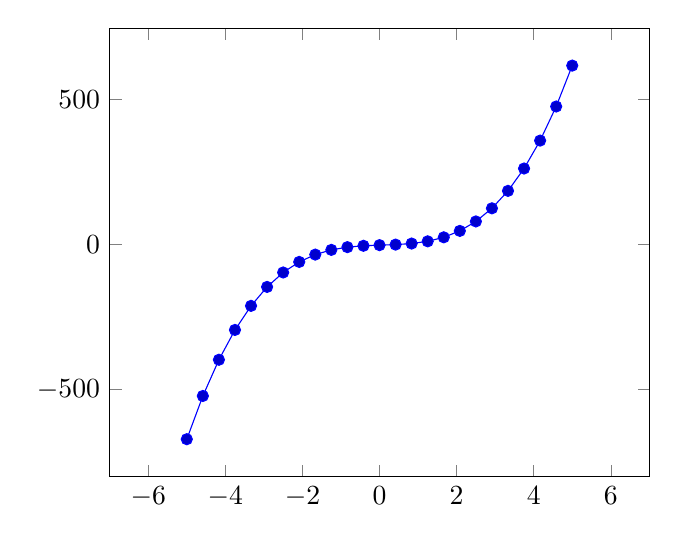
\begin{tikzpicture}
	\begin{axis}
		\addplot {5 * x^3 - x^2 + 4*x -2};
	\end{axis}
\end{tikzpicture}
\end{codeexample}

\begin{codeexample}[]
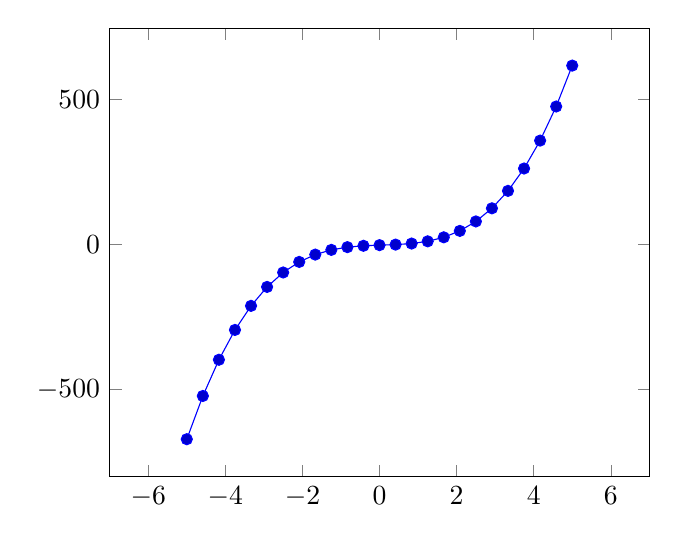
\begin{tikzpicture}
	\begin{axis}[enlarge x limits=0.2]
		\addplot {5 * x^3 - x^2 + 4*x -2};
	\end{axis}
\end{tikzpicture}
\end{codeexample}

\begin{codeexample}[]
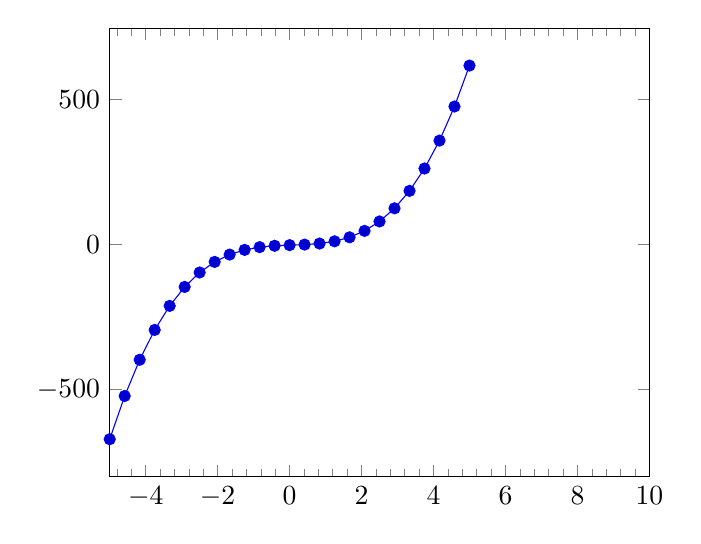
\begin{tikzpicture}
	\begin{axis}[minor x tick num=4,
		enlarge x limits={rel=0.5,upper}
	]
		\addplot {5 * x^3 - x^2 + 4*x -2};
	\end{axis}
\end{tikzpicture}
\end{codeexample}

\begin{codeexample}[]
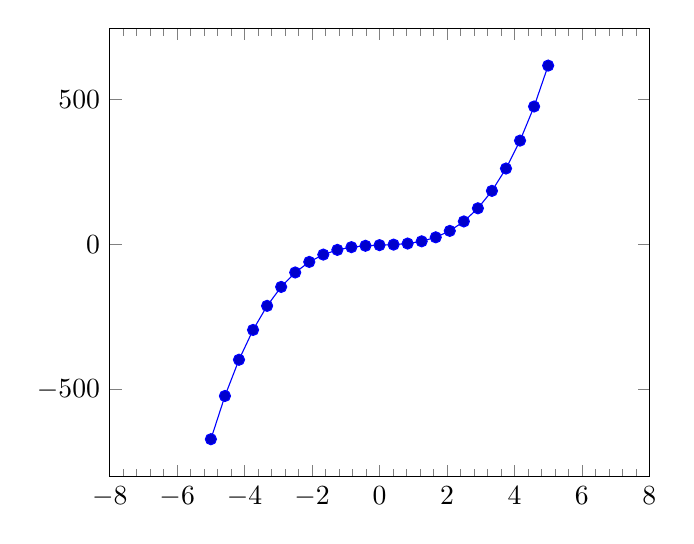
\begin{tikzpicture}
	\begin{axis}[minor x tick num=4,
		enlarge x limits={abs=3}
	]
		\addplot {5 * x^3 - x^2 + 4*x -2};
	\end{axis}
\end{tikzpicture}
\end{codeexample}

\begin{codeexample}[]
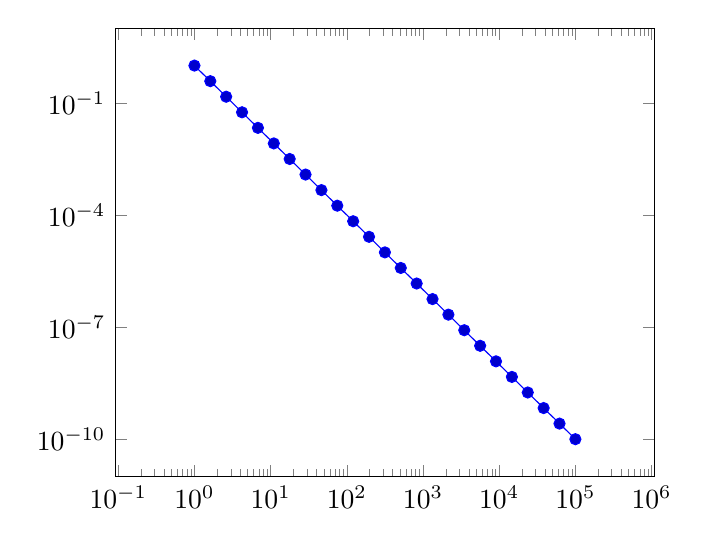
\begin{tikzpicture}
	\begin{loglogaxis}[enlarge x limits={abs=11}]
		\addplot+[domain=1:100000] {x^-2};
	\end{loglogaxis}
\end{tikzpicture}
\end{codeexample}

\end{pgfplotsxykeylist}

\begin{environment}{{pgfplotsinterruptdatabb}}
\index{Bounding Box Control!Disable \protect\emph{data} bounding box modifications}
	Everything in \marg{environment contents} will not contribute to the data bounding box.
\end{environment}
